\chapter{Resultados}

Este capítulo têm como objetivo apresentar as estratégias usadas para projetar e refinar o controle PID empregado no ajuste automático da luminosidade no modo "Econômico", mostrar o comportamento do controlador diante de algumas métricas comumente usadas para avaliar sistema de controle como sua resposta ao degrau e integral do erro, e apresentar valores estimados de consumo de energia em cenários de uso com os modos "Normal" e "Econômico". 
% Talvez não seja necessário falar isso daqui pra baixo
A demonstração das outras funcionalidades do sistema (ligar e desligar via internet, por exemplo) são triviais para que sejam mostradas de forma escrita.

\section{Sintonia e Ajustes do controle de luminosidade}

Para sintonizar as constantes do controlador PID foi utilizada a técnica de Ziegler-Nichols. Dado um porto de partida da sintonia, alguns ajustes foram feitos de forma empírica visando minimizar o \textit{overshoot}, o tempo de subida e as oscilações em regime permanente.

O método de Ziegler-Nichols é um método empírico de caracterização da planta e determinação dos parâmetros do controlador PID. O método consiste, como descrito anteriormente, na obtenção de dois parâmetros da planta: O ganho crítico, denotado por $K_{cr}$, e o período de oscilação crítico, $T_{cr}$. Os parâmetros obtidos foram:
\begin{equation}
    \label{eq:rs1}
    K_{cr} = 1.6
\end{equation}
\begin{equation}
    \label{eq:rs1.1}
    T_{cr} = 3 s.
\end{equation}

O desempenho do controlador foi avaliado para as três sintonias mais comuns oriundas do método de Ziegler-Nichols de acordo  com a Tabela \ref{ZN}.

\begin{table}[htb]
    \centering
    \caption{Resultados de sintonia de Ziegler-Nichols}
    \label{ZNvalores}
    \begin{tabular}{llll}
    \hline
    Tipo            & $K_P$ & $K_I$ & $K_D$ \\ 
    \hline \hline
    Clássico        & $0,72$ & $0,64$ & $0.36$ \\ 
    \hline
    Overshoot baixo & $0,53$ & $0,64$ & $0,96$ \\ 
    \hline
    Sem overshoot   & $0,32$ & $0,64$ & $0,96$ \\
    \hline
    \end{tabular}
\end{table}

Os comportamentos obtidos de resposta ao degrau do controlador com as sintonias listadas na Tabela \ref{ZNvalores} podem ser observados nas Figuras \ref{znclass}, \ref{znpo} e \ref{znso} respectivamente.
\begin{figure}[htb]
    \begin{center}
    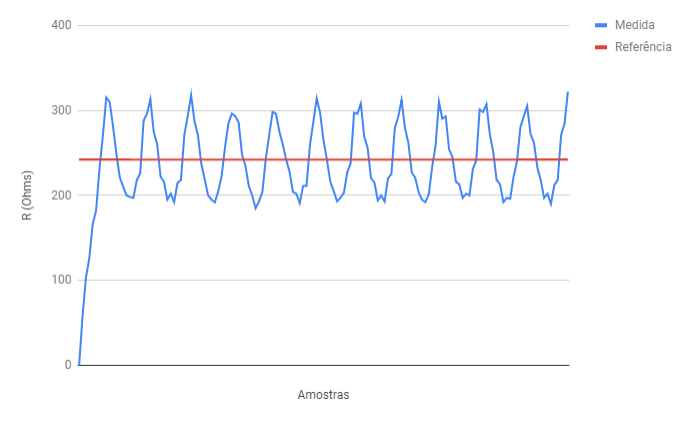
\includegraphics[width=0.75\textwidth]{figuras/znclass.PNG}
    \end{center}
    \caption[Gráfico da sintonia clássica de Ziegler-Nichols.]{Gráfico da resposta ao degrau da sintonia clássica de Ziegler-Nichols com alta oscilação em regime permanente.}
    \label{znclass}
\end{figure}
\begin{figure}[htb]
    \begin{center}
    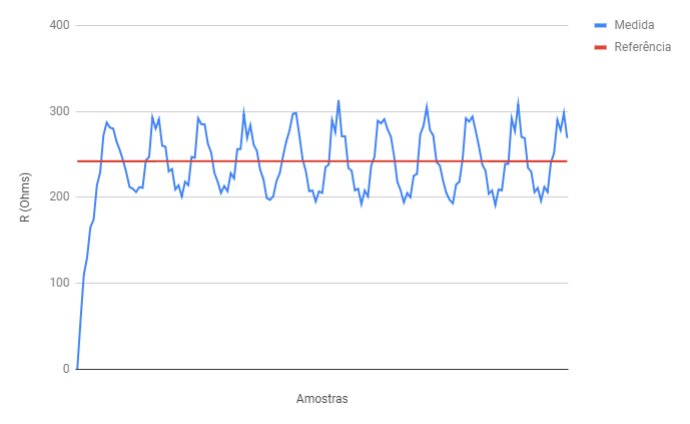
\includegraphics[width=0.75\textwidth]{figuras/znpo.PNG}
    \end{center}
    \caption[Gráfico da sintonia de Ziegler-Nichols "com pouco overshoot".]{Gráfico da resposta ao degrau da sintonia de Ziegler-Nichols "com pouco overshoot", ainda assim com alta oscilação em regime permanente.}
    \label{znpo}
\end{figure}
\begin{figure}[htb]
    \begin{center}
    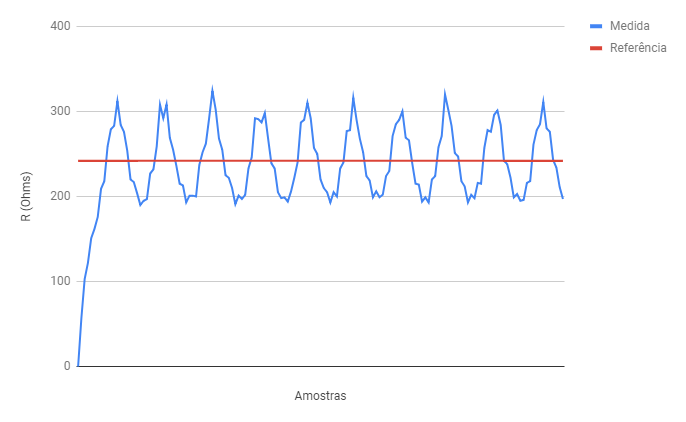
\includegraphics[width=0.75\textwidth]{figuras/znso.PNG}
    \end{center}
    \caption[Gráfico da sintonia de Ziegler-Nichols "sem overshoot".]{Gráfico da resposta ao degrau da sintonia de Ziegler-Nichols "sem overshoot", ainda assim com alta oscilação em regime permanente.}
    \label{znso}
\end{figure}

Pode-se notar que as sintonias citadas aplicadas ao controlador PID apresentam comportamento instável já que a oscilação em regime permanente não converge a zero. Tendo em vista o forte comportamento oscilatório, os ganhos integral e derivativo foram diminuídos ao ponto que o comportamento oscilatório não era mais observado, dando ao controlador um comportamento sub-amortecido, e em seguida o ganho proporcional foi incrementado até observar o aparecimento de \textit{overshoot}. A sintonia obtida nesta situação pode ser observada na Figura \ref{znsint}. 
\begin{align}
  &K_P = 1 \nonumber\\
  &K_I = 0,08 \nonumber\\
  &K_D = 0,16. \nonumber
\end{align}

\begin{figure}[htb]
    \begin{center}
    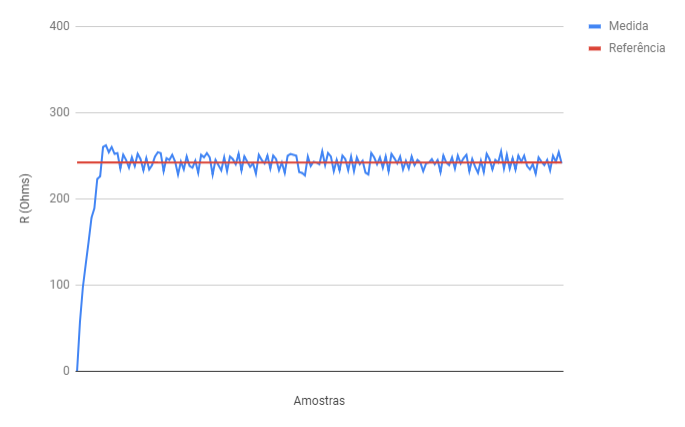
\includegraphics[width=0.75\textwidth]{figuras/znsint.PNG}
    \end{center}
    \caption[Gráfico do controlador PID satisfatoriamente sintonizado.]{Gráfico da resposta ao degrau do controlador PID satisfatoriamente sintonizado.}
    \label{znsint}
\end{figure}

\section{Desempenho do controle de luminosidade}

Outros dois experimentos foram projetados para demonstrar o comportamento do sistema de controle de luminosidade. O primeiro consiste na mudança do referencial de forma arbitrária com cinco passos discretos de valores de resistência entre 9 k$\Omega$ e 5 k$\Omega$. O segundo experimente consiste em variar a iluminação externa de forma arbitrária 

% \section{Economia de Energia}
